% Options for packages loaded elsewhere
\PassOptionsToPackage{unicode}{hyperref}
\PassOptionsToPackage{hyphens}{url}
\PassOptionsToPackage{dvipsnames,svgnames,x11names}{xcolor}
%
\documentclass[
  letterpaper,
  DIV=11,
  numbers=noendperiod]{scrartcl}

\usepackage{amsmath,amssymb}
\usepackage{iftex}
\ifPDFTeX
  \usepackage[T1]{fontenc}
  \usepackage[utf8]{inputenc}
  \usepackage{textcomp} % provide euro and other symbols
\else % if luatex or xetex
  \usepackage{unicode-math}
  \defaultfontfeatures{Scale=MatchLowercase}
  \defaultfontfeatures[\rmfamily]{Ligatures=TeX,Scale=1}
\fi
\usepackage{lmodern}
\ifPDFTeX\else  
    % xetex/luatex font selection
\fi
% Use upquote if available, for straight quotes in verbatim environments
\IfFileExists{upquote.sty}{\usepackage{upquote}}{}
\IfFileExists{microtype.sty}{% use microtype if available
  \usepackage[]{microtype}
  \UseMicrotypeSet[protrusion]{basicmath} % disable protrusion for tt fonts
}{}
\makeatletter
\@ifundefined{KOMAClassName}{% if non-KOMA class
  \IfFileExists{parskip.sty}{%
    \usepackage{parskip}
  }{% else
    \setlength{\parindent}{0pt}
    \setlength{\parskip}{6pt plus 2pt minus 1pt}}
}{% if KOMA class
  \KOMAoptions{parskip=half}}
\makeatother
\usepackage{xcolor}
\setlength{\emergencystretch}{3em} % prevent overfull lines
\setcounter{secnumdepth}{-\maxdimen} % remove section numbering
% Make \paragraph and \subparagraph free-standing
\makeatletter
\ifx\paragraph\undefined\else
  \let\oldparagraph\paragraph
  \renewcommand{\paragraph}{
    \@ifstar
      \xxxParagraphStar
      \xxxParagraphNoStar
  }
  \newcommand{\xxxParagraphStar}[1]{\oldparagraph*{#1}\mbox{}}
  \newcommand{\xxxParagraphNoStar}[1]{\oldparagraph{#1}\mbox{}}
\fi
\ifx\subparagraph\undefined\else
  \let\oldsubparagraph\subparagraph
  \renewcommand{\subparagraph}{
    \@ifstar
      \xxxSubParagraphStar
      \xxxSubParagraphNoStar
  }
  \newcommand{\xxxSubParagraphStar}[1]{\oldsubparagraph*{#1}\mbox{}}
  \newcommand{\xxxSubParagraphNoStar}[1]{\oldsubparagraph{#1}\mbox{}}
\fi
\makeatother


\providecommand{\tightlist}{%
  \setlength{\itemsep}{0pt}\setlength{\parskip}{0pt}}\usepackage{longtable,booktabs,array}
\usepackage{calc} % for calculating minipage widths
% Correct order of tables after \paragraph or \subparagraph
\usepackage{etoolbox}
\makeatletter
\patchcmd\longtable{\par}{\if@noskipsec\mbox{}\fi\par}{}{}
\makeatother
% Allow footnotes in longtable head/foot
\IfFileExists{footnotehyper.sty}{\usepackage{footnotehyper}}{\usepackage{footnote}}
\makesavenoteenv{longtable}
\usepackage{graphicx}
\makeatletter
\def\maxwidth{\ifdim\Gin@nat@width>\linewidth\linewidth\else\Gin@nat@width\fi}
\def\maxheight{\ifdim\Gin@nat@height>\textheight\textheight\else\Gin@nat@height\fi}
\makeatother
% Scale images if necessary, so that they will not overflow the page
% margins by default, and it is still possible to overwrite the defaults
% using explicit options in \includegraphics[width, height, ...]{}
\setkeys{Gin}{width=\maxwidth,height=\maxheight,keepaspectratio}
% Set default figure placement to htbp
\makeatletter
\def\fps@figure{htbp}
\makeatother

\usepackage{physics}
\newcommand{\Lagr}{\mathcal{L}}
\usepackage{tikz}
\usepackage{amsmath}
\usepackage{pgfplots}
\usepackage{caption}
\KOMAoption{captions}{tableheading}
\makeatletter
\@ifpackageloaded{caption}{}{\usepackage{caption}}
\AtBeginDocument{%
\ifdefined\contentsname
  \renewcommand*\contentsname{Table of contents}
\else
  \newcommand\contentsname{Table of contents}
\fi
\ifdefined\listfigurename
  \renewcommand*\listfigurename{List of Figures}
\else
  \newcommand\listfigurename{List of Figures}
\fi
\ifdefined\listtablename
  \renewcommand*\listtablename{List of Tables}
\else
  \newcommand\listtablename{List of Tables}
\fi
\ifdefined\figurename
  \renewcommand*\figurename{Figure}
\else
  \newcommand\figurename{Figure}
\fi
\ifdefined\tablename
  \renewcommand*\tablename{Table}
\else
  \newcommand\tablename{Table}
\fi
}
\@ifpackageloaded{float}{}{\usepackage{float}}
\floatstyle{ruled}
\@ifundefined{c@chapter}{\newfloat{codelisting}{h}{lop}}{\newfloat{codelisting}{h}{lop}[chapter]}
\floatname{codelisting}{Listing}
\newcommand*\listoflistings{\listof{codelisting}{List of Listings}}
\makeatother
\makeatletter
\makeatother
\makeatletter
\@ifpackageloaded{caption}{}{\usepackage{caption}}
\@ifpackageloaded{subcaption}{}{\usepackage{subcaption}}
\makeatother

\ifLuaTeX
  \usepackage{selnolig}  % disable illegal ligatures
\fi
\usepackage{bookmark}

\IfFileExists{xurl.sty}{\usepackage{xurl}}{} % add URL line breaks if available
\urlstyle{same} % disable monospaced font for URLs
\hypersetup{
  pdftitle={Microeconomia 1 (Lista 1)},
  pdfauthor={Frederico Fonseca Ribeiro},
  colorlinks=true,
  linkcolor={blue},
  filecolor={Maroon},
  citecolor={Blue},
  urlcolor={Blue},
  pdfcreator={LaTeX via pandoc}}


\title{Microeconomia 1 (Lista 1)}
\author{Frederico Fonseca Ribeiro}
\date{}

\begin{document}
\maketitle


\section{Questão 1}\label{questuxe3o-1}

\begin{enumerate}
\def\labelenumi{\arabic{enumi}.}
\tightlist
\item
  COMPLETUDE: O indivíduo consegue formar uma relação de preferência
  entre todas as
  cestas.(\(\forall x, y \in X, \quad x \succeq y \quad \text{ou} \quad y \succeq x\))
\item
  TRANSITIVIDADE: A relação de preferência entre as cestas consumidas é
  coerente.
  (\(\forall x, y, z \in X, \quad x \succeq y \land y \succeq z \Rightarrow x \succeq z\))
\item
  DESEJABILIDADE/MONOTONICIDADE: Também tido como Não-Saciedade: quanto
  mais,
  melhor.(\(\forall x, y \in X, \quad \left[ x_i \geq y_i \ \forall i \ \text{e} \ \exists j: x_j > y_j \right] \Rightarrow x \succ y\))
\item
  CONVEXIDADE: A média é preferível aos
  extremos.(\(\forall x, y \in X, \quad x \succeq y \text{ e } x \succeq z \Rightarrow x \succeq \lambda y + (1 - \lambda)z, \quad \forall \lambda \in [0,1]\))
\item
  CONTINUIDADE: Permite traçar relações de
  utilidade.(\(\text{Para todo } x \in X, \text{ os conjuntos } \{ y \in X : y \succeq x \} \text{ e } \{ y \in X : x \succeq y \} \text{ são fechados.}\))
\end{enumerate}

\section{Questão 2}\label{questuxe3o-2}

\subsection{a)}\label{a}

\[
UMg_1 = \frac{\partial u}{\partial x_1} = x_2
\] De forma semelhante, , encontramos a utilidade maginal de \(x_2\) e
temos que a \(TMgS = \frac{UMg_1}{UMg_2} = \frac{x_2}{x_1}\)

\subsection{b)}\label{b}

De forma semelhante, temos que: \[
TMgS = \frac{2 x_1 x^2}{2 x_1^2 x_2}
\]

\subsection{c)}\label{c}

\[
TMgS = \frac{1/x_1}{1/x_2}
\]

\section{Questão 3}\label{questuxe3o-3}

\subsection{a)}\label{a-1}

Demonstrando homogeneidade de grau zero:

\begin{align}
x_1(p,w) &= x(kp, kw) \\
\left( \frac{2w}{2p_1 + p_2} \right) &= \left( \frac{k2w}{k2p_1 + kp_2} \right) \\
&= \left( \frac{k(ww)}{k(2p_1 + p_2)} \right) \\
&= \left( \frac{2w}{2p_1 + p_2} \right)
\end{align}

Demonstrando Lei de Walras:

\begin{align}
px &= w \\
p_1x_1 + p_2x_2 &= w \\
p_1 \left(\frac{2w}{2p_1 + p_2} \right) + p_2 \left(\frac{w}{2p_1 + p_2} \right) &= w \\
w \left(\frac{2p_1 + p_2}{2p_1 + p_2}\right) &= w \\
w &= w
\end{align}

\section{b)}\label{b-1}

Demonstrando grau de homogeneidade 0 para \(x_1\), sendo os outros casos
análogos:

\begin{align}
x_1(p,w) &= x(kp, kw) \\
\left(\frac{p_2w}{(p_1+p_2+p_3)p_1}\right) &= \left(\frac{kp_2kw}{(kp_1+kp_2+kp_3)kp_1}\right) \\
&= \left(\frac{k^2p_2w}{k^2(p_1+p_2+p_3)p_1}\right) \\
&= \left(\frac{p_2w}{(p_1+p_2+p_3)p_1}\right)
\end{align}

Demonstrando Lei de Walras

\begin{align}
w &= px \\
 &=  p_1 \left(\frac{p_2w}{(p_1+p_2+p_3)p_1}\right) + p_2\left(\frac{p_3w}{(p_1+p_2+p_3)p_2}\right) +
p_3 \left(\frac{\beta p_1w}{(p_1+p_2+p_3)p_3}\right) \\
&= \left(\frac{p_2w + p_3w + \beta p_1w}{p_1 + p_2 + p_3}\right) \\
&= \frac{w(\beta p_1 + p_2 +  p_3)}{p_1 + p_2 +  p_3} \\
&= w \textnormal{, se $\beta$ = 1}
\end{align}

\section{Questão 4}\label{questuxe3o-4}

Provando homogeneidade de grau zero: \begin{align}
x_1(kp, kw) &= \frac{kp_2}{kp_3} = \frac{p_2}{p_3} = x_1(p,w) \\
x_2(kp, kw) &=- \frac{kp_1}{kp_3} = - \frac{p_1}{p_3} = x_2(p,w) \\
x_3(kp, kw) &= \frac{kw}{kp_3} = \frac{w}{p_3} = x_3(p,w)
\end{align} Provando Lei de Walras:

\[
p_1 \left(\frac{p_2}{p_3}\right) + p_2 \left(-\frac{p_1}{p_3}\right) + p_3 \left(\frac{w}{p3}\right) = w 
\] Os dois primeiros termos se anulam e os \(p_3\) também se anulam no
terceiro termo, sendo assim:

\[
w = w
\]

\section{Questão 5}\label{questuxe3o-5}

\subsection{Cobb-Douglas}\label{cobb-douglas}

\subsubsection{a)}\label{a-2}

Para mostrar que que é homotética, deve-se provar a homogeneidade de
grau 1:

\begin{align}
tu(x_1, x_2) &= u(tx_1, tx_2) \\
&= u(K(tx_1)^\alpha (tx_2)^{1-\alpha}) \\
&= Kt^\alpha x_1^\alpha t^{1-\alpha}x_2^{1-\alpha} \\
&= tKx_1^\alpha x_2^{1-\alpha}
\end{align}

\subsubsection{b)}\label{b-2}

Para encontrar a demanda Walrasiana, ou seja, em função de \(p\) e de
\(w\), devemos maximizar a função sujeita à restrição orçamentária,
sendo assim temos o seguinte lagrangeano:

\begin{equation}\phantomsection\label{eq-lagrcd}{
\mathcal{L} = Kx_1^\alpha x_2^{1-\alpha} + \lambda(w - p_1x_1 - p_2x_2)
}\end{equation}

Sendo assim, temos as seguintes condições de primeira ordem:

\begin{equation}\phantomsection\label{eq-dvx1cb}{
\pdv{\Lagr}{x_1} = \alpha Kx_1^{\alpha-1}x_2^{1-\alpha} - \lambda p_1 = 0
}\end{equation}

\begin{equation}\phantomsection\label{eq-dvx2cb}{
\pdv{\Lagr}{x_2} = (1-\alpha)Kx_1^\alpha x_2^{-\alpha} - \lambda p_2 = 0
}\end{equation}

\begin{equation}\phantomsection\label{eq-dvwcb}{
\pdv{\Lagr}{\lambda} = w - p_1x_1 - p_2x_2 = 0
}\end{equation}

Isolando \(\lambda\) e substituindo dentro de Equação~\ref{eq-dvx1cb},
temos que:

\[
K\alpha x_1^{\alpha -1}x_2^{1-\alpha} = p_1 \left(\frac{(1-\alpha)Kx_1^\alpha x_2^{-\alpha}}{p_2}  \right)
\] Podemos eliminar \(K\) dos dois lados. Além disso, para isolar
\(x_2\), dividimos ambos os lados por \(x_1^{\alpha -1}\) e
multiplicamos por \(x_2^{\alpha}\), restando:

\begin{equation}\phantomsection\label{eq-dmx2}{
x_2 = \frac{p_1}{p_2}\frac{(1-\alpha)}{\alpha}x_1
}\end{equation}

Substituindo na Equação~\ref{eq-dvwcb}, temos que:

\[
w - p_1x_1 - p_2\left( \frac{p_1}{p_2}\frac{(1-\alpha)}{\alpha}x_1\right) 
\]

\[
p_1x_1 + \left( p_1\frac{(1-\alpha)}{\alpha}x_1\right)=   w
\] \[
p_1x_1 \left(1 + \frac{(1-\alpha)}{\alpha}  \right) = w
\] \[
p_1x_1 \frac{1}{\alpha}   = w
\] E chegamos à demanda Walrasiana de \(x_1\):

\begin{equation}\phantomsection\label{eq-dmwx1}{
x_1^*(p,w) = \frac{w \alpha}{p_1}
}\end{equation}

Similarmente, encontramos \(x_2^*(p,w)\):

\begin{equation}\phantomsection\label{eq-dmwx2}{
x_2^*(p,w) = \frac{w (1-\alpha)}{p_2}
}\end{equation}

\subsubsection{c)}\label{c-1}

Para encontrarmos a função de utilidade indireta, precisamos substituir
a demanda Walrasiana dentro da função utilidade:

\[
v(p, w) =   Kw\left(\frac{w\alpha}{p_1}  \right)^\alpha \left(\frac{w(1-\alpha)}{p_2}  \right)^{1-\alpha}
\]

\subsubsection{d)}\label{d}

\subsubsection{e)}\label{e}

Para acharmos a demanda Hicksiana, devemos minimizar o gasto em função
da utilidade, sendo assim, temos:

\[
\mathcal{L} = p_1x_1 + p_2x_2 + \lambda(u - Kx_1^\alpha x_2^{-\alpha})
\] Condições de primeira ordem:

\begin{equation}\phantomsection\label{eq-dvhx1cb}{
\pdv{\Lagr}{x_1} = p_1 + \lambda K\alpha x_1^{\alpha-1}x_2^{1-\alpha} = 0
}\end{equation} \begin{equation}\phantomsection\label{eq-dvhx2cb}{
\pdv{\Lagr}{x_2} = p_2 + \lambda K(1-\alpha) x_1^{\alpha}x_2^{-\alpha} = 0
}\end{equation} \begin{equation}\phantomsection\label{eq-dvhlcb}{
\pdv{\Lagr}{\lambda} = u - Kx_1^\alpha x_2^{-\alpha}) = 0
}\end{equation}

Isolando \(\lambda\) na Equação~\ref{eq-dvhx2cb} e substituindo na
Equação~\ref{eq-dvhx1cb}, temos:

\[
p_1 - \frac{p_2hK\alpha x_1^{\alpha-1}x_2^{1-\alpha}}{K(1-\alpha) x_1^{\alpha}x_2^{-\alpha}} =
p_1 - \frac{p_2\alpha x_1^{-1}x_2^1}{(1-\alpha)} = 0
\] Isolando \(x_2\):

\begin{equation}\phantomsection\label{eq-dmx2hcb}{
x_2 = \frac{p_1}{p_2}\frac{(1-\alpha)}{\alpha}x_1
}\end{equation}

Substituindo a Equação~\ref{eq-dmx2hcb} na Equação~\ref{eq-dvhlcb}:

\[
u - Kx_1^\alpha\left(\frac{p_1}{p_2}\frac{1-\alpha}{\alpha}x_1\right)^{1-\alpha} = 0
\] Isolando \(x_1\):

\begin{equation}\phantomsection\label{eq-dhh1cb}{
x_1 = \frac{u}{K}\left(\frac{p_2}{p_1}\frac{\alpha}{1-\alpha}\right)^{1-\alpha} = h_1^*(p,u)
}\end{equation} Semelhantemente, encontra-se
\(h_2^* =  \frac{u}{K}\left(\frac{p_1}{p_2}\frac{1-\alpha}{\alpha}\right)^{\alpha}\)

\subsubsection{f)}\label{f}

Para achar a função dispêndio, basta substituir a demanda Hicksiana
dentro:

\begin{align}
e(p, u) &= p_1 \frac{u}{K} \left[ \frac{\alpha}{1 - \alpha}   \frac{p_2}{p_1} \right]^{1 - \alpha} 
+ p_2   \frac{u}{K} \left[ \frac{1 - \alpha}{\alpha}   \frac{p_1}{p_2} \right]^{\alpha} \\
&= \frac{u}{K} p_1^{\alpha} p_2^{1 - \alpha} 
\left[ \frac{\alpha^{1 - \alpha}}{(1 - \alpha)^{1 - \alpha}} + \frac{(1 - \alpha)^{\alpha}}{\alpha^{\alpha}} \right] \\
&= \frac{u}{K} p_1^{\alpha} p_2^{1 - \alpha} 
\left[ \alpha^{-\alpha} (1 - \alpha)^{-(1 - \alpha)} \right]
\end{align}

\subsubsection{g)}\label{g}

Aplicando o Lema de Shephard, basta derivar a função dispêndio em
relação ao preço:

\[
\frac{\partial e(p,u)}{\partial p_1} = \frac{u}{K}\left(\frac{p_2}{p_1}\frac{\alpha}{1-\alpha}\right)^{1-\alpha} = h_1^*(p,u)
\] Nota: o expoente \(\alpha\) que desce multiplicando ajuda na
simplificação ao evidenciar o expoente dos parênteses dos termos à
direita.

\subsubsection{h)}\label{h}

Para encontrar os efeitos Renda, Substituição e Total, devemos usar a
Equação de Slutsky.

\subsection{CES}\label{ces}

\section{Questão 6}\label{questuxe3o-6}

Podemos definir a renda real como \(R = w - p_0x\). A partir da
Equação~\ref{eq-dmwx1}, temos que:

\[
x-x_0 = \frac{R\alpha}{p_x} =\frac{( w - px_0)\alpha}{p_x}
\] Ou seja, como se gasta primeiro com \(x_0\), há uma redução da reta
orçamentária real.

\section{Questão 7}\label{questuxe3o-7}

\subsection{a)}\label{a-3}

Para resolver a questão, devemos utilizar a Identidade de Roy, sendo
assim:

\[
x_1^*(p,w) = -\frac{-\alpha/p_1}{(\alpha + \beta)/w} = \frac{\alpha}{(\alpha+\beta)}\frac{w}{p_1}
\] Similarmente, para \(x_2\):

\[
x_2^*(p,w) =  \frac{\beta}{(\alpha+\beta)}\frac{w}{p_2}
\]

\subsection{b)}\label{b-3}

Para encontrar a função dispêndio, basta isolar \(w\):

\[
\ln w = \frac{\alpha\ln p_1 + \beta\ln p_2 -K+u}{(\alpha + \beta)}
\] Usando propriedades logarítimicas e depois usando função exponencial,
tem-se que:

\[
e(p, u) = e^{\frac{u - K}{\alpha + \beta}} p_1^{\frac{\alpha}{\alpha + \beta}} p_2^{\frac{\beta}{\alpha + \beta}}
\] Para chegar à Demanda Hicksiana, aplica-se o Lema de Shephard, que é
a derivação da função dispêndio pelo preço:

\[
h_1(p, u) = \frac{\alpha}{\alpha + \beta} \, e^{\frac{u - K}{\alpha + \beta}} \left( \frac{p_2}{p_1} \right)^{\frac{\beta}{\alpha + \beta}}
\] Semelhantemente, para o outro bem:

\[
h_2(p, u) = \frac{\beta}{\alpha + \beta} \, e^{\frac{u - K}{\alpha + \beta}} \left( \frac{p_1}{p_2} \right)^{\frac{\alpha}{\alpha + \beta}}
\]

\section{Questão 8}\label{questuxe3o-8}

\subsection{a)}\label{a-4}

Para esta questão, considere \(\alpha = 1/2\)

Logo, a fim de maximizar a utilidade dada uma restrição orçamentária,
temos as seguintes CPOs:

\[
\alpha x_1^{\alpha-1} + \lambda p_1 = 0
\] \[
(1-\alpha) x_2^{-\alpha} + \lambda p_2 = 0
\] \[
w - p_1x_1 - p_2x_2 = 0
\] Igualando as equações, temos que:

\[
\frac{(1-\alpha) x_2^{-\alpha}}{p_2} = \frac{\alpha x_1^{\alpha-1}}{p_1}
\] Isolando:

\[
x_2^\alpha = \frac{p_1}{p_2}\frac{\alpha}{(1-\alpha)}x_1^{\alpha-1}
\] \[
x_2 = \left(\frac{p_1}{p_2}\frac{\alpha}{(1-\alpha)x_1^{1-\alpha}}\right)^\frac{1}{\alpha}
\] Reduzindo ao substituir \(\alpha\):

\[
x_2 = \left(\frac{p_1}{p_2}\right)^2x_1
\] Substituindo na restrição orçamentária:

\[
w = p_1x_1 + p_2\left(\frac{p_1}{p_2}\right)^2x_1
\] \[
x_1^* = \frac{w}{p_1+\frac{p_1^2}{p_2}}
\] \[
x_1^* = \frac{p_2w}{p_1p_2+p_1^2}
\] Similarmente: \[
x_2^* = \frac{p_1w}{p_1p_2+p_2^2}
\] Substituindo na função utilidade:

\[
v(p^*, w) = \left(\frac{p_1w}{p_1p_2+p_2^2}\right)^{1/2} + \left(\frac{p_2w}{p_1p_2+p_1^2}\right)^{1/2}
\] \[
v(p^*, w) = w^{1/2}\left(\frac{p_1^2+p_2^2}{p_1p_2(p_1+p_2)}\right)^{1/2}
\]

Para achar a função dispêndio, deve-se isolar \(w\): \[
w = u^2\left(\frac{p_1p_2(p_1+p_2)}{(p_1+p_2)^2}\right)
\]

\[
w = u^2\left(\frac{p_1p_2}{(p_1+p_2)}\right)
\] Da função dispêndio, derivando em relação aos preços, encontra-se a
Demanda Hicksiana:

Dica: Em vez de usar regra do quociente, bote a expressão em baixo
elevado a -1 para usar a regra do produto.

\[
u^2 \left[ 
p_2  (p_1 + p_2)^{-1}- p_1p_2(p_1 + p_2)^{-2}\right] = u^2\frac{p_2^2}{(p_1 + p_2)^2} =
h_1(p,u)
\] Semelhantemente para o bem 2:

\[
u^2\frac{p_1^2}{(p_1 + p_2)^2} = h_2(p,u)
\]

\subsection{b)}\label{b-4}

Para responder, devemos utilizar a Equação de Slutsky:

Para achar \(ET\), basta a diferença de \(x_2\) com os diferentes
preços:

\[
\frac{1\cdot 10}{2 \cdot 1 + 2^2} - \frac{1 \cdot 10}{1 \cdot 1 + 1^2}
\] \[
\frac{10}{6}-\frac{10}{2} = \frac{-10}{3} = ET
\] Efeito renda, sendo a derivada da demanda walrasiana em relação a
\(w\):

\[
-\frac{p_2}{p_1p_2 + p_2^2}x_1
\] Sendo assim, temos: \[
-\frac{1}{2 \cdot 1 + 1^2}\cdot \frac{1 \cdot 10}{2 \cdot 1 + 2^2} = -\frac{1}{3}\frac{10}{6} = 
-\frac{5}{9} = ER
\] Sendo assim, o \(ES = ET - ER\) é igual a:

\[
-\frac{10}{3}-\left(-\frac{5}{9}\right)
\] \[
\frac{5}{9}-\frac{30}{9} = -\frac{25}{9} = ES
\]

\section{Questão 9}\label{questuxe3o-9}

\subsection{a)}\label{a-5}

Dado um aumento de renda, a demanda do bem \(x\) aumentará se for um bem
normal e o oposto, caso for um bem inferior.

Em relaçao à \(TMgS\), caso a renda aumente, o valor continuará o mesmo,
apenas mudando a curva de indiferença em que a escolha ótima está, mas
com a inclinação da reta constante.

\begin{center}
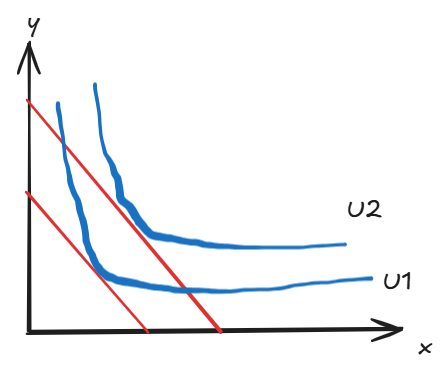
\includegraphics{aumentorenda.png}
\end{center}

Já para as Curvas de Engel, tem-se:

\begin{center}
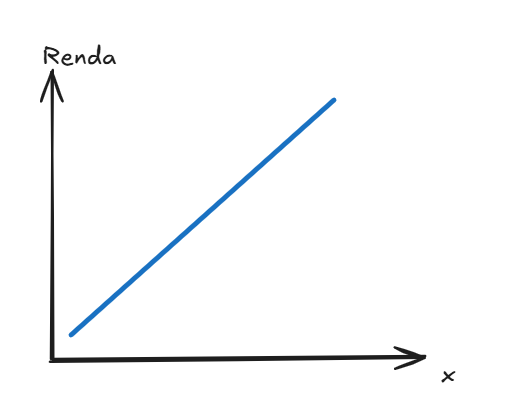
\includegraphics{engelnormal.png}
\end{center}
Quanto maior a renda, maior a demanda de \(x\).

\begin{center}
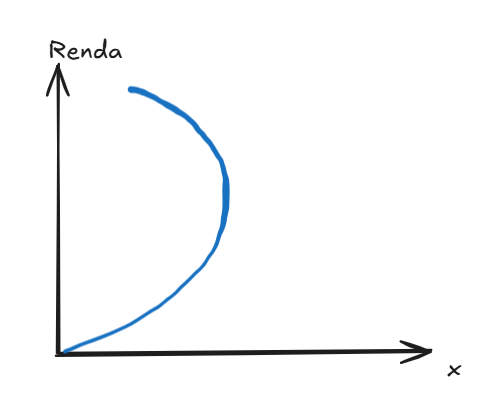
\includegraphics{engelinferior.png}
\end{center}
Para um bem inferior, após certo ponto da renda, a demanda diminui.

\subsection{b)}\label{b-5}

Ao aumentar o preço, há o efeito substituição e o efeito renda. O de
substituição se refere ao aumento da demanda de outro bem, vide a
relação cruzada de demanda e preço. Já o efeito renda, se refere ao
impacto do preço na renda real.

\section{Questão 10}\label{questuxe3o-10}

O resultado esperado de cada loteria se dá por:

\[
L_1 = \left(0\cdot \frac{1}{3} + 100 \cdot \frac{1}{3} + 200 \cdot \frac{1}{3}\right) = 100
\] \[
L_2 = \left(0\cdot \frac{1}{2} + 100 \cdot 0 + 200 \cdot \frac{1}{2}\right) = 100
\] \[
L_3 = \left(0\cdot 0 + 100 \cdot \frac{3}{4} + 200 \cdot \frac{1}{4}\right) = 125
\] Assumindo uma relação linear tal qual \(u(x) = x\), tanto o valor
esperado de \(L_2\) quanto de \(L_3\) são maiores que \(L_1\), logo há
contradição.

\section{Questão 11}\label{questuxe3o-11}

\subsection{a)}\label{a-6}

\[
r_A(x)= - \frac{-\frac{1}{4}x^{-3/2}}{\frac{1}{2}x^{-1/2}}
\] \[
r_A(x)= \frac{1}{2x}
\] Substituindo \(x\):

\[
\frac{1}{2 \cdot 5} = 0,1
\] Relativa:

\[
R_R = 5 \cdot 0,1 = 0,5
\]

\subsection{b)}\label{b-6}

Primeiro devemos calcular a utilidade esperada:

\[
\mathbb{E}(u) = \sqrt{16} \cdot \frac{1}{2} + \sqrt{4}\cdot \frac{1}{2} = 3
\] Achando o Equivalente Certeza:

\[
EC = 3^2 = 9
\] Prêmio de Probabilidade:

\[
\sqrt{10} =   \sqrt{16} \cdot \left(\frac{1}{2}- \pi\right) + \sqrt{4}\cdot \left(\frac{1}{2}+ \pi\right)
\] Isolando \(pi\):

\[
\sqrt{10} = 4 \cdot \left(\frac{1-2\pi}{2}\right) + 2\cdot \left(\frac{1+2\pi}{2} \right)
\]

\[
\sqrt{10} = 2(1-2\pi) + (1+2\pi)
\] \[
\sqrt{10} = 2-4\pi +1 +2\pi
\] \[
\frac{\sqrt{10} - 3}{2}
\] Por que a renda inicial é 10? Não tem no enunciado. PERGUNTAR

\subsection{c)}\label{c-2}

Achando a utilidade esperada: \[
\mathbb{E}(u) = \sqrt{36} \cdot \frac{1}{2} + \sqrt{16}\cdot \frac{1}{2} = 5
\] Achando \(EC\):

\[
EC = 5^2 = 25
\] De forma semelhante à letra anterior, tem-se o prêmio de
probabilidade:

\[
\sqrt{26} = 6 \cdot \left(\frac{1+2\pi}{2}\right) + 4\cdot \left(\frac{1-2\pi}{2} \right)
\] \[
\sqrt{26}= 3+6\pi + 2 - 4\pi
\] \$\$ \pi = \frac{\sqrt{26} - 5}{2}

\$\$ \# Questão 12

\section{Questão 13}\label{questuxe3o-13}

\section{Questão 14}\label{questuxe3o-14}

\section{Questão 15}\label{questuxe3o-15}




\end{document}
